% !TeX spellcheck = da_DK
\section{Apopleksi}
Hjernen har brug for ilt og næringsstoffer for at kunne fungere normalt og er derfor afhængig af en kontant blodgennemstrømning. Hvis denne tilstrømning stopper, kan det have alvorlige konsekvenser. \cite{Hjernesagen2015a} Apopleksi er en sygdom, som har stor indvirkning på blodgennemstrømningen til hjernen. Sundhedsstyrelsen definerer apopleksi som pludseligt opståede fokalneurologiske symptomer af formodet vaskulær genese med en varighed på over 24 timer. \cite{Sundhedsstyrelsen2009} Hvis varigheden er under 24 timer, betegnes det som transitorisk cerebral iskæmi (TCI), hvor de fleste tilfælde varer under 1 time uden permanent hjerneskade \cite{Sundhed.dk2014, Ritter2015}. Disse korte tilfælde kaldes forbigående blodpropper i hjernen, og flere tusinde danskere oplever dem årligt, men det er sjældent at folk selv er klar over det. Symptomerne heraf er meget milde og kan være en følelsesløshed i lemmerne eller i ansigtet samt korte oplevelser af forvirring, synsforstyrrelser og sproglige forstyrrelser. Det er sjældent, at der opstår mén fra disse tilfælde og derfor kræves der ikke behandling. \cite{Hjernesagen2015a,Academic2015} 
%Symptomerne heraf er meget milde, og selvom man ikke får behandling for disse forbigående blodpropper i hjernen, er det sjældent, at der opstår mén fra tilfældet. [7] 
Symptomerne på apopleksi kan fremtræde efter et par minutter, men der kan også gå op til et par dage før de fremtræder \cite{Kruuse2014, Academic2015}.
%Derudover kan der opstå mere alvorlige tilfælde af apopleksi, hvor det i værste tilfælde vil føre til koma eller død [11].
Årsagerne til apopleksi kan være forhøjet blodtryk, rygning, højt kolesteroltal, diabetes og arvelige defekter. Konsekvenserne fra apopleksi kan omfatte forbigående eller varig lammelse af forskellige dele af kroppen, %på en eller begge sider af kroppen, 
vanskeligheder ved tale, vanskeligheder ved spisning og et tab i muskuløs koordinering. \cite{Academic2015} Hurtig behandling er essentielt for at mindske disse konsekvenser. Hver fjerde apopleksi patient er imidlertid afhængig af andres hjælp i hverdagen. \cite{Hjernesagen2015a} \\ %(døde dele af hjernevæv)
Et apopleksi tilfælde kan være forårsaget af enten en blodprop i hjernen (iskæmisk) eller hjerneblødning (hæmoragisk).\fxnote{det her skal skrives om, så parenteserne bliver ophævet} \cite{Ritter2015} 

\begin{figure}[H]
	\centering
	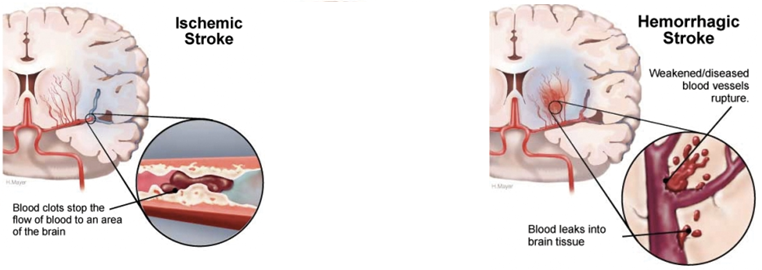
\includegraphics[scale=0.8]{figures/bProblemanalyse/haemoragisk_og_iskaemisk.png}
	\caption{På billedet ses, hvad der sker i hjernen, når henholdsvis iskæmisk og hæmoragisk apoplekså opstår. Der ses til venstre, at iskæmisk apopleksi sker, hvis en hjerneartierie blokkes. Til højre ses, at hæmoragisk apopleksi opstår, når en hjernearterie brister.\cite{Ritter2015}}
	\label{haem-isk}
\end{figure}

\subsubsection{Iskæmisk apopleksi}
Iskæmisk apopleksi opstår i 80-85\% af tilfældene iblandt det samlede antal af apopleksi ramte \cite{Sundhed.dk2014}. Her blokeres en hjernearterie af en blodprop, der stopper tilførslen af blod til et bestemt område i hjernen, hvilket ses på \figref{haem-isk}. Infarkterne dannes primært pga. åreforkalkning enten ved en trombe, der dannes på stedet, eller emboli fra hjertet. \cite{Schulze2011} Emboli består typisk af fragmenter af blodceller eller kolesterol, som er diffunderet ind i blodcirkulationen af hjernen fra en arterierne \cite{Academic2015a}. En alvorlig blødning et andet sted på kroppen kan også resultere i blokeret eller stoppet blodtilførsel til hjernen. \cite{Hjernesagen2015a} Nervecellerne skades efter få minutter grundet iltmangel, men kan i værste tilfælde fuldstændig dø efter denne periode \cite{Schulze2011,Giraldo2015}.% grundet iltmangel efter få minutter, og hvis dette fortsætter i en periode, vil de til sidst gå tabt. [5] % Specificer denne periode - hvor lang tid går der, før nervecellen går tabt?

\subsubsection{Hæmoragisk apopleksi}
Hæmoragisk apopleksi opstår i 10-15\% af tilfældene iblandt det samlede antal af apopleksiramte \cite{Sundhed.dk2014}. Årsagen heraf skyldes hovedsagligt forhøjet blodtryk eller, i sjældnere tilfælde, bristede svagheder på arterier eller medfødte misdannede kar \cite{Schulze2011}. Hæmoragisk apopleksi opstår, når en hjernearterie brister og lækage af blod danner en blodansamling, der beskadiger det omkringliggende væv og forøger trykket i hjernen, hvilket ses på \figref{haem-isk}. Intracerebral hæmoragi kommer af forhøjet blodtryk, der danner et pres på de små arterier, som får dem til at briste. \cite{Caplan2006} \\
Blødning i subaraknoidalrummet skyldes bristning af en aneurisme i en pulsåre i hjernen \cite{Schulze2011}. Symptomerne ved subaraknoidalblødning er generel tab af hjernefunktion, da der forekommer et øget pres på hjerneskallen, hvorimod ved intracerebral hæmoragi er hæmatomet lokaliseret et bestemt sted i hjernen og forårsager nedsat funktion ved én bestemt hjernefunktion \cite{Caplan2006}. 





%%%%%%%%%%%%%%%%%%%%%%%%%%%%%%%%%%%%%%%%%%%%%%%%%%%%                KILDER                 %%%%%%%%%%%%%%%%%%%%%%%%%%%%%%%%%%%%%%%%%%%%%%%%%%%%%%
% [1] = https://sundhedsstyrelsen.dk/da/udgivelser/2010/~/media/1A28F73140B54143B490B89DD687E3C9.ashx
% [2]: https://www.sundhed.dk/sundhedsfaglig/laegehaandbogen/hjerte-kar/tilstande-og-sygdomme/apopleksi-og-tia/apopleksi-og-tia-tci/#1 
% [3]: http://heart.arizona.edu/heart-health/preventing-stroke/lowering-risks-stroke 
% [4]: http://site.ebrary.com/lib/aalborguniv/reader.action?docID=10130864 (søgeord: hemorrage apoplexy)
% [5]: basisbog i sygdomslære: https://books.google.dk/books?id=vNK8CRu4t9sC&pg=PA444&lpg=PA444&dq=karokklusion&source=bl&ots=jAu__8N4Oz&sig=I4LKVLfRFQVE4NZYjHpUepM6jms&hl=da&sa=X&ved=0CEMQ6AEwB2oVChMI1Lbp_fv4xwIVCANzCh0AmgAV#v=onepage&q=apopleksi&f=false 
% [6]: Britannica - http://academic.eb.com.zorac.aub.aau.dk/EBchecked/topic/569347/stroke
% [7]: Hjernesagen - http://www.hjernesagen.dk/om-hjerneskader/bloedning-eller-blodprop-i-hjernen/fakta-om-apopleksi]
% [8]: Britannica - http://academic.eb.com.zorac.aub.aau.dk/EBchecked/topic/1800831/nervous-system-disease/75792/Stroke?anchor=ref606262
% [9]: http://www.merckmanuals.com/home/brain-spinal-cord-and-nerve-disorders/stroke-cva/overview-of-stroke
% [10] https://www.sundhed.dk/borger/sygdomme-a-aa/hjerte-og-blodkar/sygdomme/apopleksi/apopleksi-blodprop-eller-bloedning-i-hjernen/
% [11] http://academic.eb.com.zorac.aub.aau.dk/EBchecked/topic/569347/stroke
% [12] http://www.netdoktor.dk/sygdomme/fakta/blodprophjerne.htm




%%%%%%%%%%%%%%%%%%%%%%%%%%%%%%%%%%%%%%%%%%%%%%%%%%%%%%%%%%%%%%%%% Gamle ting
%Apopleksi er af World Health Organization (WHO) defineret som pludseligt opstået fokale neurologiske symptomer pga. forstyrrelser i hjernens blodcirkulation, der varer mere end 24 timer eller fører til døden[1gammel].
% [1gammel] = (Experience from a multicentre stroke register: a preliminary report.): http://www.ncbi.nlm.nih.gov/pubmed?cmd=Search&term=Bull%20WHO%20%5Bta%5D%20AND%2054%5Bvol%5D%20AND%20541%5Bpage%5D 